\documentclass{beamer}
\usetheme{}
\usecolortheme{dolphin}           
\useinnertheme{circles}
\setbeamertemplate{itemize items}[default]
\setbeamertemplate{enumerate items}[default]
\usepackage[T1]{fontenc}
\usepackage[utf8]{inputenc}
\usepackage{lmodern}
\usepackage{amsmath}
\usepackage{booktabs} 
\usepackage{graphicx}        
\usepackage{array}
\usepackage{color}
\makeatletter
\def\zapcolorreset{\let\reset@color\relax\ignorespaces}
\def\colorrows#1{\noalign{\aftergroup\zapcolorreset#1}\ignorespaces}
\makeatother
\setbeamertemplate{navigation symbols}{}
\setbeamertemplate{footline}[frame number]

%--------------------------------------
\title{Macroeconomic integration}
\author{School of Economics, University College Dublin}
\date{Spring 2018}
\begin{document}

%--------------------------------------
\begin{frame}
 \titlepage
\end{frame}
%--------------------------------------

%--------------------------------------
\begin{frame}
  \textbf{Balassa}
  \begin{enumerate}
    \item Preferential customs area
    \item Free trade area
    \item Customs union
    \item Common market
    \item Economic and monetary union
    \item Political union
  \end{enumerate}
\end{frame}
%--------------------------------------

%--------------------------------------
\begin{frame}
  EU currently at stage 4/5
  \begin{itemize}
    \item All member countries part of the common market
    \item Some member of a monetary union (eurozone)
  \end{itemize}
  \medskip
  Members of the eurozone can set \textbf{fiscal} policy but not \textbf{monetary} policy
  \begin{itemize}
    \item Autonomy over public spending and taxing
    \item Can't set interest rates or depreciate/appreciate currency
  \end{itemize}
\end{frame}
%--------------------------------------

%--------------------------------------
\begin{frame}
  Recent crisis exposed current shortcomings concerning integration; specifically of monetary union
  \begin{enumerate}
    \item Abolish euro: move back to stage 4
    \item Further integration: moving towards stage 6
    \begin{enumerate}[i]
      \item Banking union (2014)
      \item Fiscal union
      \item Political union
    \end{enumerate}    
  \end{enumerate}  
\end{frame}
%--------------------------------------

%--------------------------------------
\begin{frame}
  \textbf{Political project}\\
  Two schools of thought on integration
  \begin{enumerate}
    \item Intergovernmentalism
    \begin{itemize}
      \item National governments are in charge
      \item States can use EU for their own goals
    \end{itemize}
    \medskip
    \item Functionalism
    \begin{itemize}
      \item Integration pushed by elites and interest groups that transcend national boundaries
      \item Dynamic effect of transferring functions from national government to Brussels
    \end{itemize}
  \end{enumerate}
\end{frame}
%--------------------------------------

%--------------------------------------
\begin{frame}
  European integration therefore either
  \begin{enumerate}
    \item Follows from national economic interests
    \medskip
    \item Or is a path towards political integration
  \end{enumerate}  
\end{frame}
%--------------------------------------

%--------------------------------------
\begin{frame}
  Functionalism works through a \textbf{chain reaction}
  \begin{enumerate}
    \item Move functions in narrow areas from government to supranational body
    \item Over time will lead to more integration 
  \end{enumerate}
  \medskip
  Further centralisation will follow through +ve/-ve mechanisms
  \begin{itemize}
    \item +ve: through learning, changing preferences
    \item -ve: generating problems and crises
  \end{itemize}
\end{frame}
%--------------------------------------

%--------------------------------------
\begin{frame}
  Further centralisation through -ve mechanism implies that national politicians don't anticipate chain reaction  
  \medskip
  \begin{enumerate}
    \item Short horizons
    \item Asymmetric information
    \item Democratic deficit
  \end{enumerate}
\end{frame}
%--------------------------------------

%--------------------------------------
\begin{frame}
  In remainder of course we will focus on
  \begin{enumerate}
    \item Monetary policy
    \item Fiscal policy
    \item Economic growth
  \end{enumerate}
  \medskip
  Start with some basic economics
\end{frame}
%--------------------------------------

%--------------------------------------
\begin{frame}
  \textbf{Closed economy}
  \begin{align}
    Y=C+I+G
  \end{align}
  \medskip
  Equilibrium GDP given by
  \begin{align}
    Y=C(Y) + I +G
  \end{align}
  \begin{enumerate}
    \item Consumers spend more when they earn more; earn more when firms produce more
    \item Firms invest borrowing at interest rate $i$; when $i$ increases, $I$ and $C$ decrease 
  \end{enumerate}  
\end{frame}
%--------------------------------------

%--------------------------------------
\begin{frame}
  \begin{align*}
    Y=C(Y) + I + G
  \end{align*}
  \medskip
  Note that government can change spending $G$
  \begin{itemize}
    \item e.g. could increase spending in infrastructure
  \end{itemize}
  \medskip
  Government spending is set by fiscal policy and this is important in context of business cycles
  \begin{itemize}
    \item Expansionary policy will increase $G$ and reduce taxes
  \end{itemize}
\end{frame}
%--------------------------------------

%--------------------------------------
\begin{frame}
  \begin{figure}
    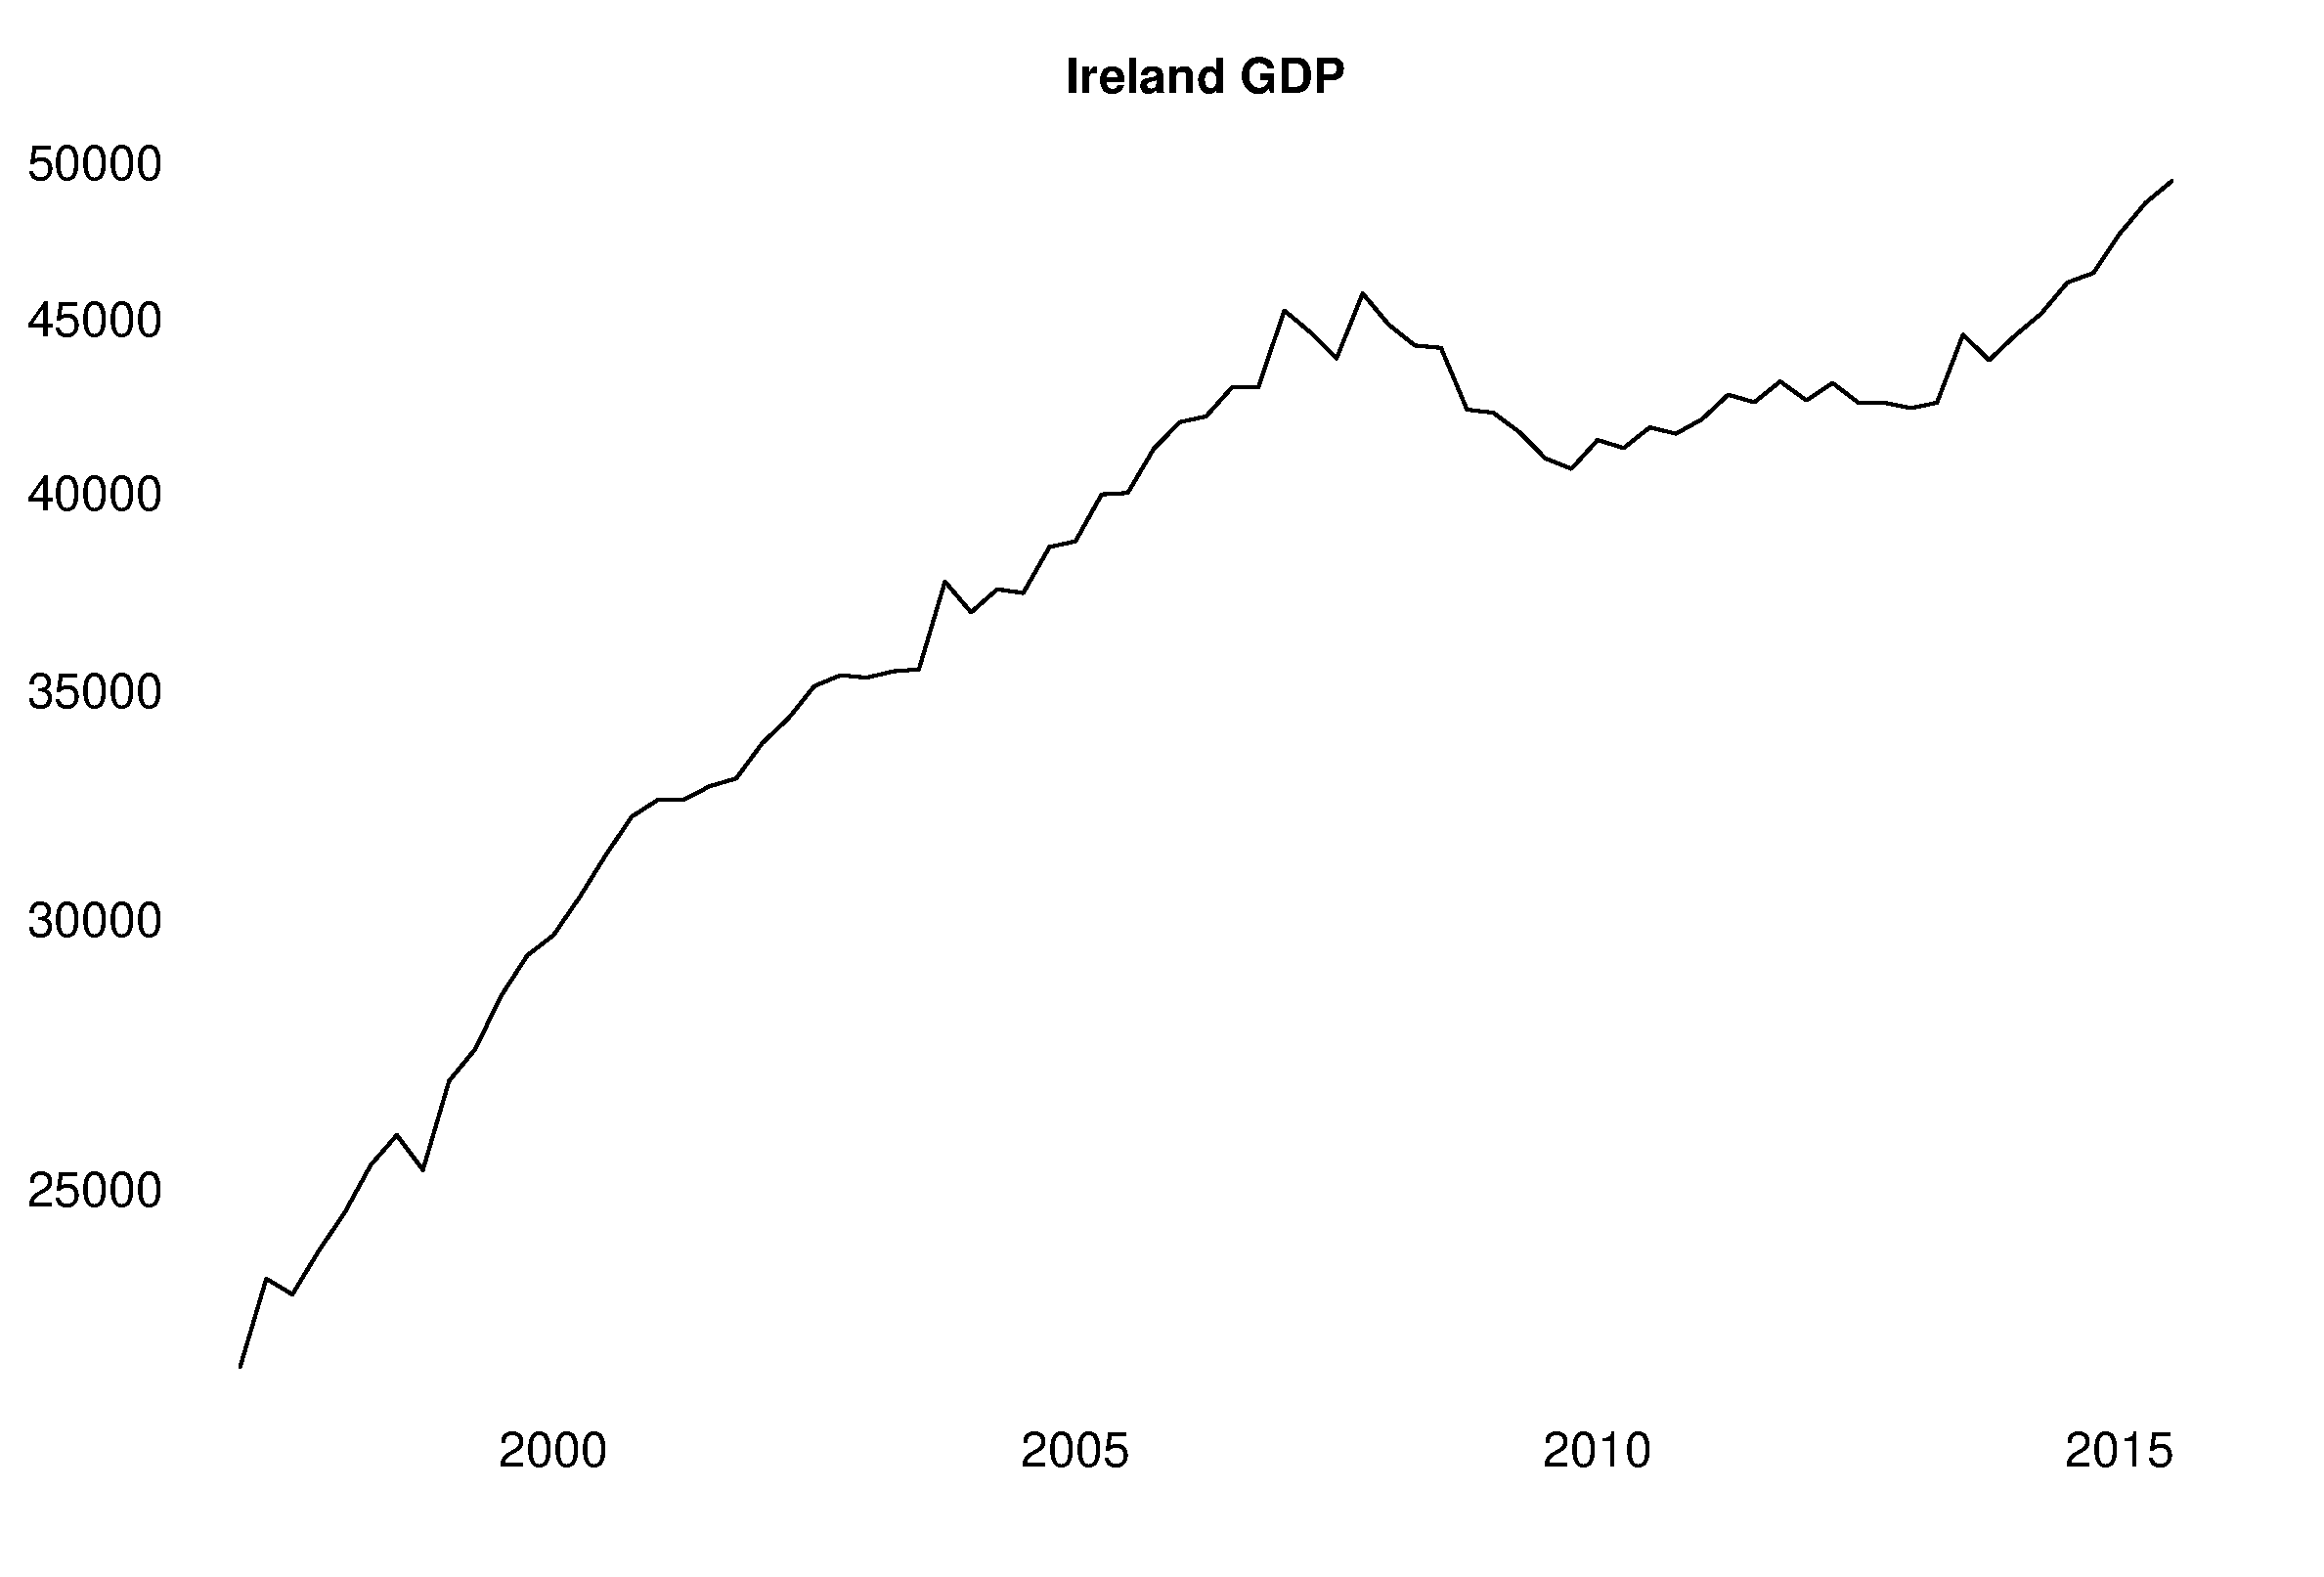
\includegraphics[scale=.25]{ire_gdp.eps}
  \end{figure}
\end{frame}
%--------------------------------------

%--------------------------------------
\begin{frame}
  \begin{figure}
    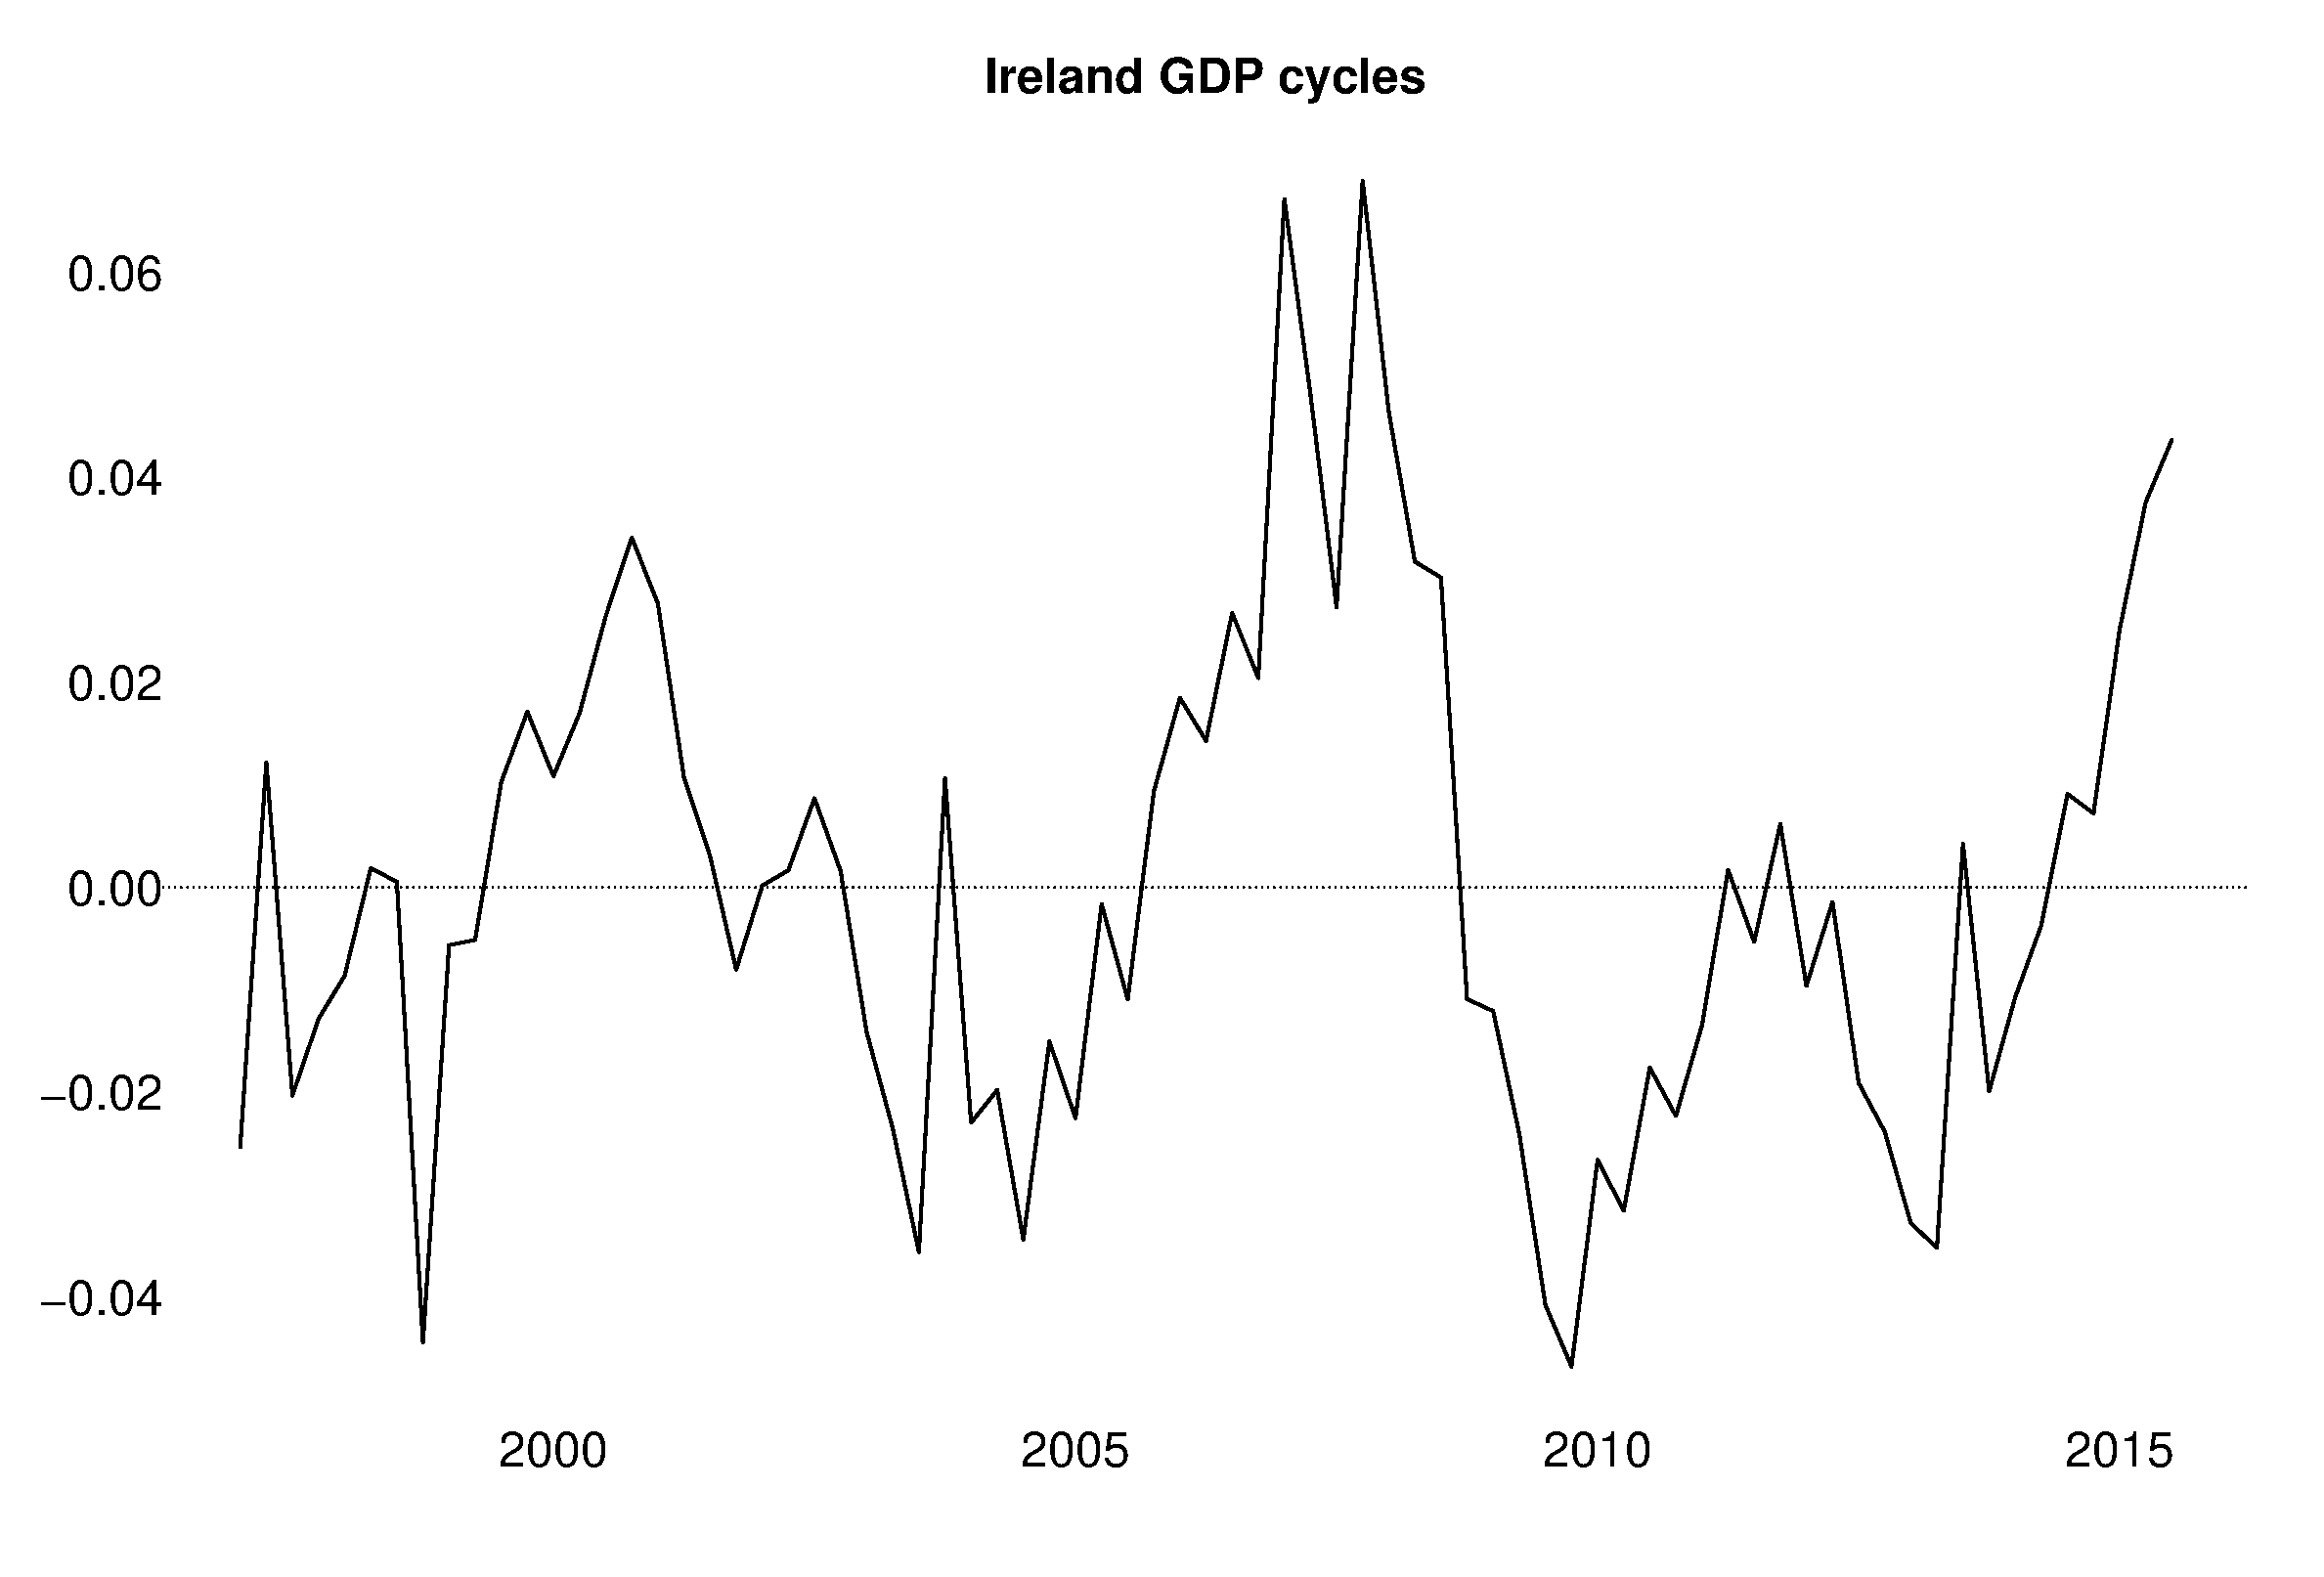
\includegraphics[scale=.25]{ire_gdp_hp.eps}
  \end{figure}
\end{frame}
%--------------------------------------

%--------------------------------------
\begin{frame}
  \begin{figure}
    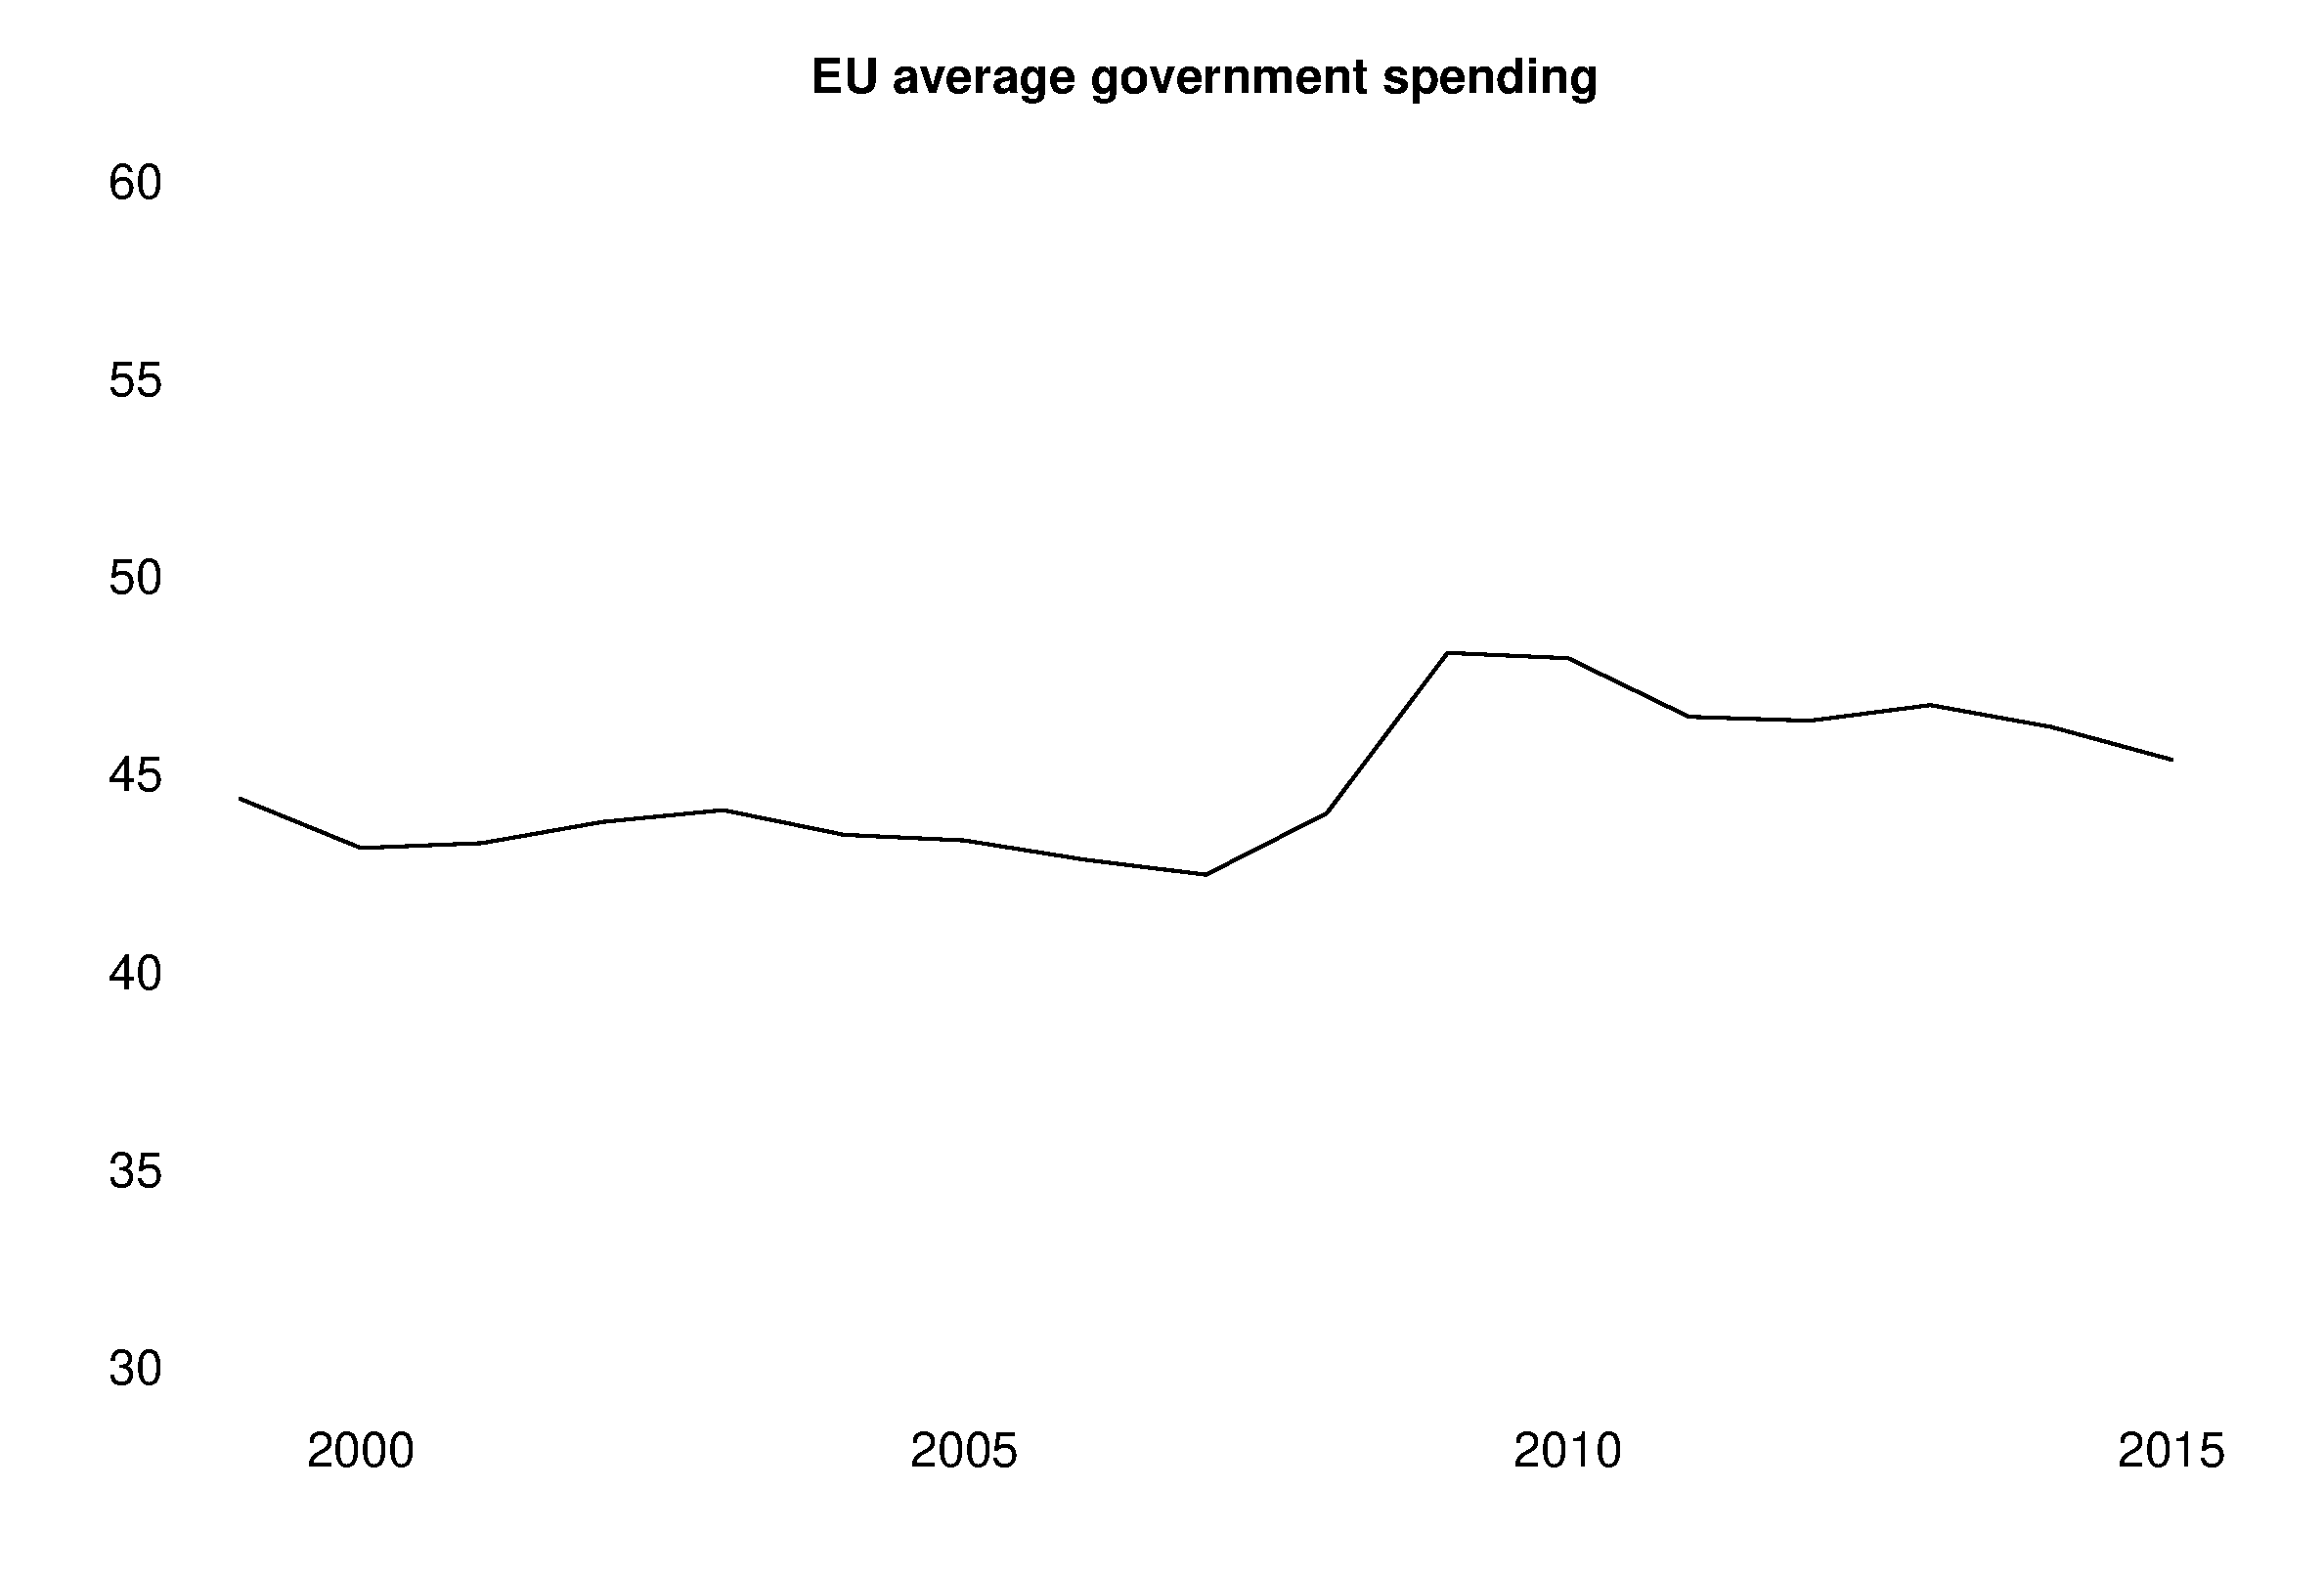
\includegraphics[scale=.2]{eu_G.eps}
  \end{figure}
\end{frame}
%--------------------------------------

%--------------------------------------
\begin{frame}
  In the economy there is an important role for \textbf{financial markets}
  \begin{itemize}
     \item Collect savings from households/firms
     \item Lend money to households/firm and public authorities
   \end{itemize} 
   \medskip
   Number of feature of the financial market that are of interest
  \begin{enumerate}
    \item Finance is associated with risk
    \item Financial intermediaries deal with each other, continuously
    \item Price associated with risk
    \item Most people rely on banks for savings deposits
  \end{enumerate}
\end{frame}
%--------------------------------------

%--------------------------------------
\begin{frame}
  Financial markets are subject to 
  \begin{enumerate}
    \item Regulations
    \item Monetary policy
  \end{enumerate}
  And monetary policy is set by central bank, which generally has two objectives
  \medskip
  \begin{enumerate}
    \item Control inflation
    \item Stabilise economy
  \end{enumerate}  
\end{frame}
%--------------------------------------

%--------------------------------------
\begin{frame}
  \textbf{Open economy}  
  \begin{align}
    Y=C+I+G+X-M
  \end{align}
  $X$ is exports\\
  $M$ is imports\\
  $X-M$ is current account.  
  \medskip
  \begin{itemize}
    \item Goods and services markets become interdependent across countries
  \end{itemize}
\end{frame}
%--------------------------------------

%--------------------------------------
\begin{frame}
  \textbf{Interest rate parity condition}
  \begin{align}
    1+i_t = (1+r^*) \frac{E^e_{t+1}}{E_t}
  \end{align}
  When exchange rate is expected to depreciate, higher interest rate is needed to prevent capital outflows
  \begin{itemize}
    \item Expected exchange rate appreciation is accompanied by lower interest rate at home compared to foreign
  \end{itemize}  
\end{frame}
%--------------------------------------

%--------------------------------------
\begin{frame}
  Can restate parity condition as
  \begin{align}
    i_t = i^*_t +  \frac{E^e_{t+1}}{E_t}
  \end{align}
  \begin{quote}
    Domestic interest rate = Foreign interest rate + Expected exchange rate depreciation
  \end{quote}
  Parity condition cannot be directly observed
  \begin{itemize}
    \item $E^e_{t+1}$ cannot be measured
    \item On whom does $E^e_{t+1}$ depend? 
  \end{itemize}  
\end{frame}
%--------------------------------------

%--------------------------------------
\begin{frame}
 Interest rate parity condition shows \textbf{market sentiment}, revealing market expectations
  \begin{align}
      \frac{E^e_{t+1}}{E_t} = i_t - i^*_t 
  \end{align} 
  Or the expected exchange rate depreciation equals Domestic interest rate minus Foreign interest rate  
\end{frame}
%--------------------------------------


%--------------------------------------
\begin{frame}
  \textbf{Impossible trinity principle}
  \begin{enumerate}
    \item Good markets equilibrium
    \item Monetary preferences
    \item Interest rate parity
  \end{enumerate}
  Can only have two out of three
  \begin{enumerate}
    \item Full capital mobility
    \item Fixed exchange rate
    \item Autonomous monetary policy
  \end{enumerate}
\end{frame}
%--------------------------------------


%--------------------------------------
\begin{frame}
  \begin{enumerate}
    \item Full capital mobility and autonomous monetary policy, flexible exchange rate
    \begin{itemize}
      \item Eurozone
      \item Volatile exchange rates could harm competitiveness
    \end{itemize}
    \item Full capital mobility and fixed exchange rate
    \begin{itemize}
      \item Bretton Woods system (1944-1973), Denmark
    \end{itemize}
    \item Fixed exchange rate and monetary policy autonomy, with capital controls
    \begin{itemize}
      \item Brazil
      \item Need to enforce restrictions
    \end{itemize}
  \end{enumerate}
\end{frame}
%--------------------------------------

%--------------------------------------
\begin{frame}
  \textbf{Prices:} Two main principles
  \begin{enumerate}
    \item Monetary neutrality
    \item Purchasing power
  \end{enumerate}
  Recall central bank setting interest rate
  \begin{itemize}
    \item Lowering interest rate encourages spending    
  \end{itemize}
  Works on short run (1-3 years), after that monetary policy loses influence. 
  \begin{itemize}
    \item Stronger demand leads to higher prices; eroding purchasing power
  \end{itemize}
  i.e. purchasing power is inversely related to price level: \textbf{Monetary neutrality}
  \begin{quote}
    In the long run, monetary policy loses its effectiveness because the price level increases in the same proportion as the money stock
  \end{quote}
\end{frame}
%--------------------------------------

%--------------------------------------
\begin{frame} 
  \textbf{Real exchange rate:} Already saw that $E$ matters for competitiveness but so should prices
  \begin{itemize}
    \item $P$, price for domestic good
    \item $P^*$, price for foreign good
  \end{itemize}
  Can define real exchange rate as
  \begin{align}
    \frac{EP}{P^*}
  \end{align}
  or relative price of domestic goods expressed in foreign goods.
  Rate appreciates when
  \begin{itemize}
    \item Nominal exchange rate $E$ appreciates
    \item $\frac{P}{P^*}$ increases, i.e. $P$ rises faster than $P^*$
  \end{itemize}
\end{frame}
%--------------------------------------

%--------------------------------------
\begin{frame}
  \textbf{Purchasing power parity principle:}Rate of change of the nominal exchange rate is equal to the difference between inflation rates in two countries.
  \begin{align}
    \frac{E_t}{E_{t-1}} = \pi^* - \pi
  \end{align}
  $\pi$ is inflation rate.
  \begin{itemize}
    \item If $\pi<\pi^*$, currency should appreciate
  \end{itemize}
  This principle only holds in the long run-when it holds!
\end{frame}
%--------------------------------------

%--------------------------------------
\begin{frame}
  \textbf{Equilibrium real exchange rate:} PPP implies that $\frac{EP}{P^*}$ is constant.
  Rate of change of real exchange rate can be given by
  \begin{align}
    \frac{\Delta \frac{EP}{P^*}}{\frac{EP}{P^*}}=  \frac{\Delta E}{E} + \frac{\Delta P}{P} - \frac{\Delta P^*}{P}
  \end{align}
  If follows that
  \begin{align}
    \frac{\Delta \frac{EP}{P^*}}{\frac{EP}{P^*}}=0
  \end{align}
  when
  \begin{align}
    \frac{\Delta E}{E} = \frac{\Delta P^*}{P^*} - \frac{\Delta P}{P}
  \end{align}
\end{frame}



%--------------------------------------
\begin{frame}   
  Consider situation appreciation of real exchange rate
  \begin{itemize}
    \item Country becomes less competitive
    \item Exports decline; domestic goods are more expensive on foreign markets
    \item Imports increase; foreign goods cheaper at home
    \item Deficit needs to be financed through borrowing abroad
  \end{itemize}
  One of two things need to occur for real exchange rate to return to equilibrium
  \begin{enumerate}
    \item Depreciation of nominal exchange rate
    \item Prices must move to re-establish competitiveness
  \end{enumerate}
\end{frame}
%--------------------------------------

%--------------------------------------
\begin{frame}
  \textbf{Balassa-Samuelson effect:}
  \begin{quote}
    Equilibrium real exchange rates of countries that enjoy lasting fast growth - because they are catching up from a lower level of development - follow an appreciating trend
  \end{quote}
  By-product of catch-up process when relatively underdeveloped countries gradually close the technology gap between themselves and advanced countries.
  \begin{itemize}
    \item $EP/P^*$ is steadily increasing as domestic prices rise relative to foreign prices evaluated in domestic currency $P^* / E$
    \item Or when domestic prices evaluated in foreign currency $EP$ rise relative to foreign prices $P^*$
  \end{itemize}
  Real appreciation can happen due to
  \begin{enumerate}
    \item Higher inflation at home: $P / P^*$ increasing
    \item Continuous nominal appreciation: rising trend in $E$
  \end{enumerate}
  or combination of these two.
\end{frame}


%--------------------------------------
\end{document}
